\documentclass[12pt,letterpaper]{article}

% --- Paquetes Requeridos ---
\usepackage[utf8]{inputenc}
\usepackage[spanish,es-tabla]{babel}
\usepackage[margin=2.5cm]{geometry}
\usepackage{graphicx}
\usepackage{float}
\usepackage{titlesec}
\usepackage{setspace}
\usepackage{hyperref}
\usepackage{booktabs}
\usepackage{caption}
\usepackage{enumitem}
\usepackage{listings}
\usepackage{xcolor}

% --- Configuración de Párrafo ---
\onehalfspacing
\setlength{\parindent}{0pt}
\setlength{\parskip}{1em}

% --- Rutas de búsqueda de imágenes ---
% Permite compilar tanto desde Documentos/Entregables/ como con todas las
% imágenes en una sola carpeta plana.
\graphicspath{{./}{../Evidencia/}{Evidencia/}{imagenes/}{../DocumentoFinal/imagenes/}}

% --- Configuración de listings ---
\lstset{
    basicstyle=\ttfamily\footnotesize,
    breaklines=true,
    frame=single,
    captionpos=b,
    showstringspaces=false
}

% --- Inicio del Documento ---
\begin{document}

% --- PORTADA ---
\begin{titlepage}
    \centering

    {\Large \textbf{UNIVERSIDAD SANTO TOMÁS}} \\[1cm]

    {\Large \textbf{Sistema colaborativo de robots móviles para asistencia de orientación en entornos interiores con múltiples pisos}} \\[2cm]

    {\large \textbf{Realizado por:}} \\
    {\large Santiago Hernández Ávila} \\
    {\large Jonny Alejandro Mejía León} \\[1cm]

    \begin{figure}[H]
        \centering
        % Logotipo de la Universidad y la Facultad (en Documentos/, o junto al .tex); si no está, el de la
        % Universidad del documento final.
        \IfFileExists{../Logos Uni.png}{
\includegraphics[width=0.6\textwidth]{../Logos Uni.png}}{%
          \IfFileExists{Logos Uni.png}{\includegraphics[width=0.6\textwidth]{Logos Uni.png}}{%
            \includegraphics[width=0.35\textwidth]{logo_usta.png}}}
        \label{Logo Universidad Santo Tomas y facultad de ingenieria electronica}
    \end{figure}

    \vfill

    {\large \textbf{Informe de Avance --- Semana 28}} \\
    {\large Fase 6: análisis y escritura} \\
    {\large Resultados en el documento final y video de la campaña} \\[1.5cm]

    \textbf{Dirigido por:} \\
    Ing. Armando Mateus Rojas, Msc. \\
    Ing. Nestor Ivan Ospina, Msc. \\
    Ing. Oscar Mauricio Gélvez Lizarazo, Msc. \\[1.0cm]

    \vfill

    {\large GED (Grupo de Estudio y Desarrollo en Robótica)} \\
    {\large Facultad de Ingeniería Electrónica} \\
    {\large División de Ingenierías} \\
    {\large Bogotá, octubre de 2026}
\end{titlepage}

% --- CONTENIDO ---

\section{Introducción}

Este informe presenta el avance de la semana 28 del cronograma (19 al 25 de octubre de 2026), la primera después del cierre de la toma de datos. El corte se adelantó al martes 20 y cubre los dos primeros días de la semana.

El trabajo fue de escritura y de documentación de la campaña del 16 de octubre. El documento final quedó con los resultados del sistema completo sobre los dos vehículos, las conclusiones de los cuatro objetivos y un recorrido del trabajo desde la plataforma DonkeyCar que proponía el anteproyecto. Se editó el video de la campaña, con la pantalla del teléfono del usuario sincronizada con lo que veía. Al sincronizarlo se encontró un dato equivocado del informe anterior, que se corrige en la sección~\ref{sec:correcciones}.

Quedan dos pendientes de la semana. Uno es la restricción RNF-03 (operación en condiciones controladas), cuya observación de las personas en el pasillo se está registrando con los videos. El otro es la prueba en un teléfono de los ajustes de la página, prevista para el jueves 23.

\section{Objetivos de la semana}

El cronograma fija para esta semana el siguiente criterio de cierre:

\begin{quote}
\textit{Sustentación realizada; observaciones del jurado registradas por escrito.}
\end{quote}

El criterio no se cumplió al corte: la sustentación no se ha realizado y su fecha la fija la Universidad, en esta semana o en la siguiente. La otra actividad de la semana, los ensayos de la demostración en vivo, tampoco se hizo. Lo que el cronograma sitúa en la semana 29, definir la estructura del documento final e iniciar su redacción, ya está hecho (sección~\ref{sec:documento}).

\section{Los dos vehículos con el código vigente}

El 19 de octubre se copiaron a los dos vehículos los cambios del 18 de octubre: los textos de la página y del coordinador con tildes, y los puntos de interés de nombre repetido con su piso (``Ascensor (piso 3)''). Los dos quedaron con los 28 archivos de coordinación iguales a los del repositorio, y la prueba del coordinador con vehículos simulados pasó 19 de 19 escenarios dentro de cada uno. Se comprobó, sin mover los vehículos, que la página se sirve sin copias guardadas en el navegador y que el catálogo muestra el piso de los ascensores.

\section{Documento final}
\label{sec:documento}

El documento compila en el equipo del proyecto: 91 páginas, sin errores ni referencias sin resolver.

\subsection{Resultados del sistema completo}

El capítulo 4 tiene una sección nueva con la misión con relevo y la campaña de nueve misiones: la tabla de cada misión, la figura con la duración de cada etapa y el criterio de conteo de los intentos. Al descomponer cada misión en etapas apareció que el intervalo del relevo (del final del primer tramo al primer movimiento del segundo vehículo), con mediana de 1,22~s, junta dos situaciones. En cinco misiones el segundo vehículo tuvo que ir a su escalera y arrancó en menos de 1,3~s. En las otras cuatro ya estaba allí, y el intervalo, de 12,9 a 27,5~s, mide sobre todo cuánto tardó la persona en confirmar. Para la persona, el tiempo entre llegar a la escalera de un piso y empezar el guiado en el otro tuvo una mediana de 24,8~s, de 18,0 a 29,5~s. Los vehículos hicieron 24 medias vueltas en las nueve misiones. Se añadió como limitación que la llegada se verificó con la localización del propio vehículo y no con una medida externa.

\subsection{Conclusiones, trabajos futuros y resumen}

Quedaron cerrados con la campaña. Los trabajos futuros suman una medida externa de la llegada y la estabilidad de la navegación en sesiones largas.

\subsection{Recorrido del trabajo}

El capítulo 3 cuenta ahora el trabajo en el orden en que se hizo. Empieza por el simulador y el modelo del DonkeyCar, con sus limitaciones. Sigue con el paso al modelo de AWS DeepRacer y su migración a ROS~2 Humble, los primeros entornos con el seguidor de paredes, la integración en simulación y el trabajo con los vehículos. La fuente es \texttt{CRONOLOGIA.md}, que reúne semana a semana los entregables 10 a 27 y los 391 cambios del repositorio \cite{cronologia}.

\subsection{Decisiones del equipo}

El antecedente que el anteproyecto atribuía a Parra Buitrago (2021) no se incluye, porque no se encontró la referencia completa. El marco legal queda con las dos políticas CONPES, la norma NTC 1486 y el alcance de la operación \cite{pendientes}.

\section{Video de la campaña}

El 16 de octubre el equipo grabó el video en primera persona (POV) de quien hacía de usuario en cada misión y la pantalla de su teléfono durante toda la sesión. En las misiones 4, 5 y 9 grabó además el vehículo del otro piso mientras iba a su escalera. Con ese material se editó un video de 12~min 40~s, a tiempo real y sin audio, con el POV a la izquierda y la pantalla del teléfono a la derecha en el mismo instante. En los relevos de las misiones 4, 5 y 9 se ven los dos POV lado a lado (figura~\ref{fig:video}).

\begin{figure}[H]
    \centering
    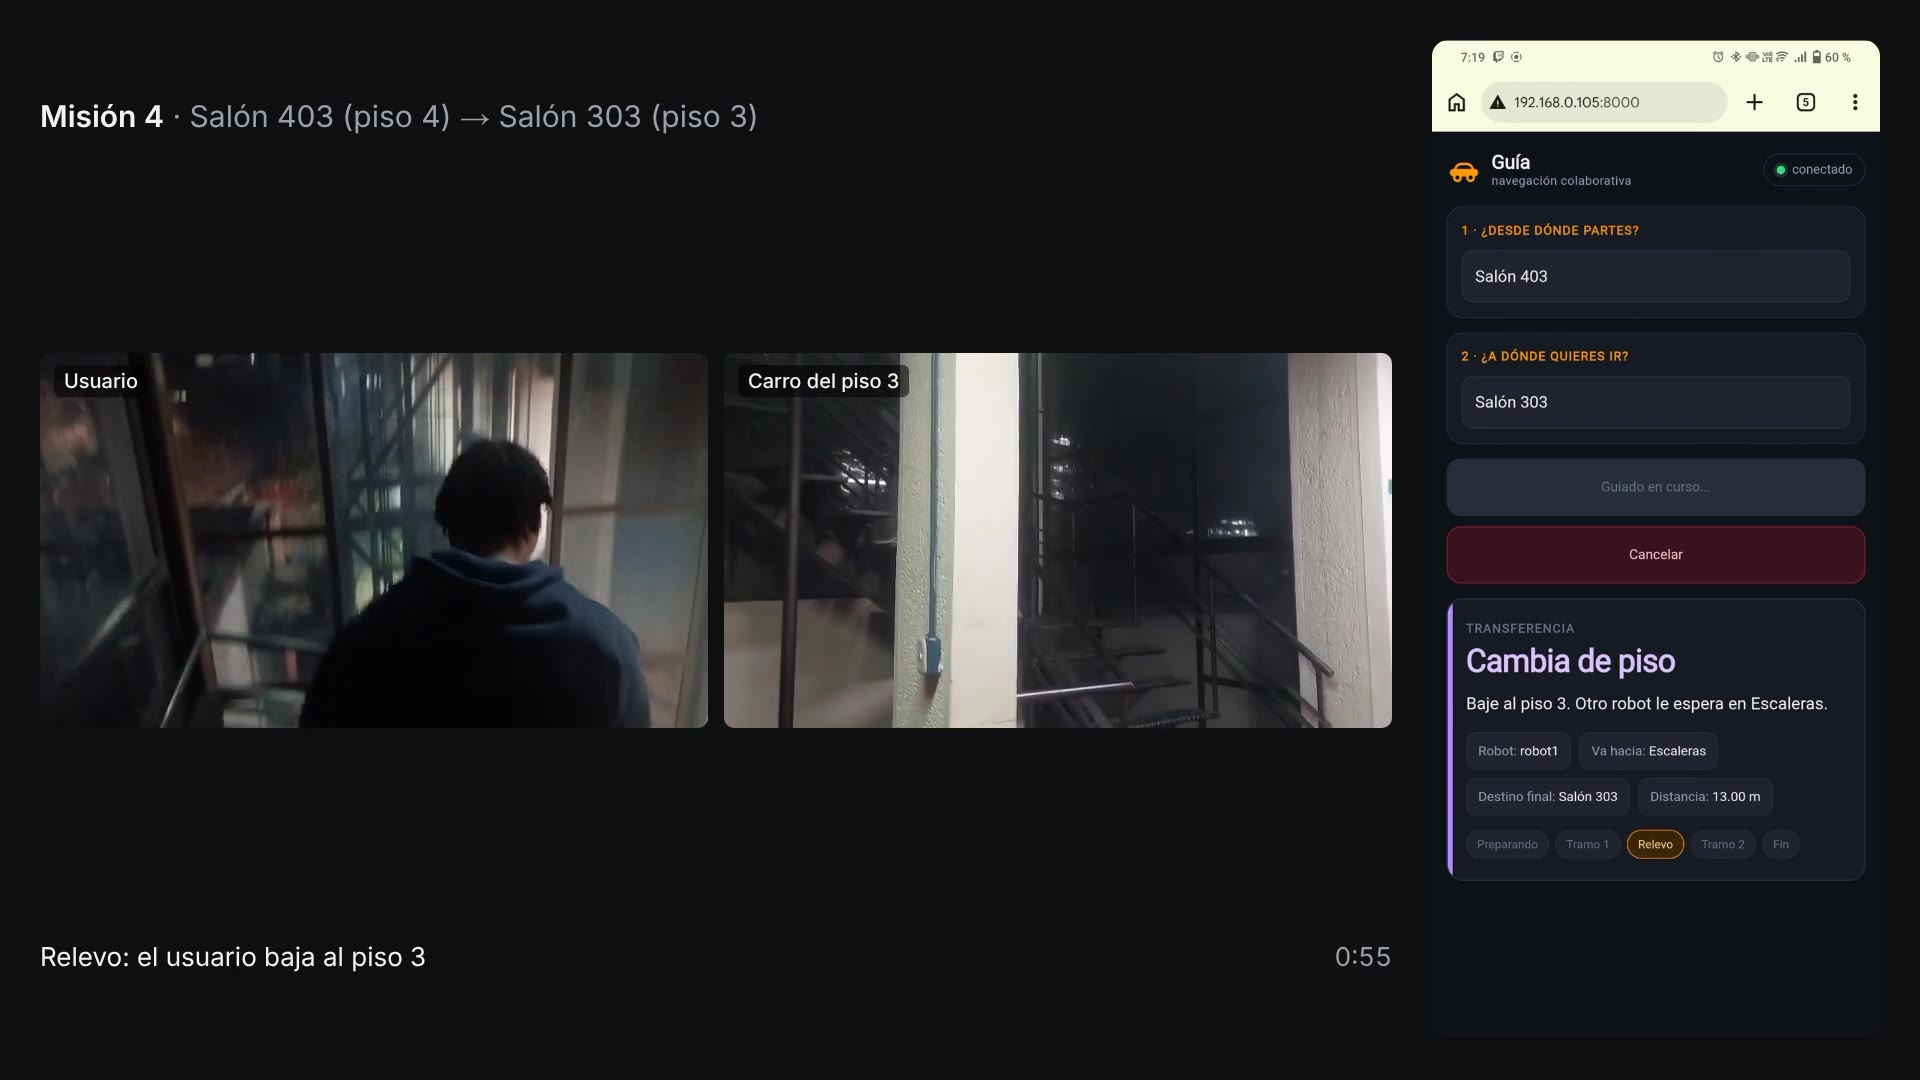
\includegraphics[width=\textwidth]{S28_video_campana_relevo.jpg}
    \caption{Relevo de la misión 4: el usuario baja por la escalera del piso 4 mientras el vehículo del piso 3 va a su escalera; el teléfono muestra ``Cambia de piso''.}
    \label{fig:video}
\end{figure}

La pantalla del teléfono se sincronizó con el coordinador por el momento en que la página muestra ``Hemos llegado'' en las diez llegadas registradas: el desfase es de 616,6~s, con $\pm$0,3~s de dispersión. Cada POV se ubicó por la hora de fin de su archivo y por el teléfono visible dentro del video. Cuatro videos tenían la escalera recortada; se sincronizaron por partes, con la pulsación de ``Pedir guía'' y la media vuelta del vehículo como referencias. El montaje se guardó también como proyecto de Shotcut, para retocarlo a mano. Los videos no se versionan en el repositorio. El método y los desfases están en \texttt{S28\_video\_campana.md} \cite{video}.

\section{Correcciones a informes anteriores}
\label{sec:correcciones}

\begin{table}[H]
\centering
\small
\caption{Dato corregido del informe de la semana 27.}
\begin{tabular}{@{}p{2.2cm}p{4.6cm}p{4.6cm}p{3.2cm}@{}}
\toprule
\textbf{Informe} & \textbf{Dato publicado} & \textbf{Dato correcto} & \textbf{Evidencia} \\ \midrule
Semana 27, sección 6 & La misión 10 no se cuenta porque ``el portátil se apagó por batería 18~s después de pedirla'' & El portátil se apagó unos 30~s después de pedirla, con el vehículo \texttt{amss-jgm9} ya en su escalera & \cite{campana}, resultado 4; \cite{video} \\ \bottomrule
\end{tabular}
\end{table}

La cifra de 18~s salía del final de la grabación de datos, que pierde su último bloque cuando el grabador se corta de golpe. La pantalla del teléfono, sincronizada, muestra la página en ``Cambia de piso'' a los 28,6~s y sin conexión con el coordinador a los 30,2~s. La misión sigue fuera del conteo.

\section{Aporte a los objetivos específicos}

\begin{table}[H]
\centering
\small
\caption{Relación entre las actividades de la semana y los objetivos específicos.}
\begin{tabular}{@{}p{4.4cm}p{1.8cm}p{8.4cm}@{}}
\toprule
\textbf{Actividad} & \textbf{Objetivo} & \textbf{Aporte} \\ \midrule
Vehículos con el código vigente & OE2, OE3 & Los dos vehículos ejecutan la versión de la página y del coordinador que usará la demostración \\
Resultados del sistema completo & OE4 & La campaña con los vehículos queda escrita en el documento final, con su limitación de medida \\
Video de la campaña & OE3, OE4 & Evidencia visual de las nueve misiones, con la interfaz del usuario sincronizada \\ \bottomrule
\end{tabular}
\end{table}

\begin{table}[H]
\centering
\small
\caption{Avance de los objetivos específicos al 20 de octubre.}
\begin{tabular}{@{}p{1.9cm}p{1.6cm}p{5.2cm}p{5.9cm}@{}}
\toprule
\textbf{Objetivo} & \textbf{Avance} & \textbf{Aporte de la semana} & \textbf{Pendiente} \\ \midrule
OE1 & 100 \% & --- & --- \\
OE2 & 100 \% & Vehículos con el código vigente & --- \\
OE3 & 100 \% & --- & Prueba de los ajustes de la página en un teléfono, el jueves 23 \\
OE4 & 100 \% & Resultados escritos en el documento final & --- \\ \bottomrule
\end{tabular}
\end{table}

El promedio de los cuatro objetivos sigue en 100~\%, frente al 87,5~\% del calendario (semana 28 de 32). De la matriz de requisitos queda parcial RNF-03, la operación en condiciones controladas, que pide registrar como observación las personas que pasaron durante las pruebas \cite{requisitos}. Los videos muestran personas en el pasillo en algunas misiones, y la observación se está registrando misión por misión.

\section{Estado del cronograma y trabajo previsto}

\begin{table}[H]
\centering
\small
\caption{Criterio de cierre de la semana 28.}
\begin{tabular}{@{}p{6cm}p{6cm}p{2.6cm}@{}}
\toprule
\textbf{Parte del criterio de cierre} & \textbf{Estado} & \textbf{Evidencia} \\ \midrule
Sustentación realizada & Pendiente de la fecha de la Universidad & --- \\
Observaciones del jurado registradas & Pendiente de la sustentación & --- \\ \bottomrule
\end{tabular}
\end{table}

Para el resto de la semana el equipo prevé:

\begin{enumerate}
    \item Registrar con los videos las personas en el pasillo durante la campaña y cerrar RNF-03.
    \item Probar el jueves 23, con un teléfono y los vehículos, los ajustes de la página.
    \item Incorporar las observaciones del jurado al documento final cuando se realice la sustentación.
\end{enumerate}

\section{Conclusiones}

\begin{enumerate}
    \item El documento final tiene redactados los resultados del sistema completo con los dos vehículos y las conclusiones de los cuatro objetivos, y compila sin errores en 91 páginas.
    \item El intervalo del relevo en los vehículos mide la reacción del sistema solo cuando el segundo vehículo tiene que ir a su escalera; cuando ya está en ella, mide la confirmación de la persona.
    \item El video de la campaña muestra las nueve misiones con la interfaz del usuario sincronizada a $\pm$0,3~s con el coordinador.
    \item El dato de la misión 10 publicado en la semana 27 estaba equivocado: el portátil se apagó unos 30~s después de la solicitud, no a los 18~s.
\end{enumerate}

\section{Anexos}

Las cifras de este informe proceden de los registros y documentos de evidencia del repositorio del proyecto, que se listan a continuación. El mismo informe está disponible en Markdown, en \texttt{Entregable\_semana\_28.md}, para leerlo directamente en el repositorio.

\begin{thebibliography}{99}

\bibitem{cronologia}
S. Hernández Ávila y J. A. Mejía León,
``Cronología del trabajo, semana a semana,''
Repositorio del proyecto, \texttt{Documentos/DocumentoFinal/CRONOLOGIA.md}, octubre de 2026.

\bibitem{pendientes}
S. Hernández Ávila y J. A. Mejía León,
``Documento final: lo que falta por completar,''
Repositorio del proyecto, \texttt{Documentos/DocumentoFinal/PENDIENTES.md}, octubre de 2026.

\bibitem{campana}
S. Hernández Ávila,
``Campaña del sistema completo con los dos vehículos, pisos 3 y 4,''
Repositorio del proyecto, \texttt{Documentos/Evidencia/S27\_campana\_rf27.md}, octubre de 2026.

\bibitem{video}
S. Hernández Ávila,
``Video de la campaña con los dos vehículos, sincronizado con la pantalla del teléfono,''
Repositorio del proyecto, \texttt{Documentos/Evidencia/S28\_video\_campana.md}, octubre de 2026.

\bibitem{requisitos}
S. Hernández Ávila y J. A. Mejía León,
``Matriz de requisitos,''
Repositorio del proyecto, \texttt{Documentos/REQUISITOS.md}, octubre de 2026.

\bibitem{cronograma}
S. Hernández Ávila y J. A. Mejía León,
``Cronograma de actividades, semanas 17 a 32,''
Repositorio del proyecto, \texttt{Documentos/CRONOGRAMA\_S17\_S32.md}, agosto de 2026.

\end{thebibliography}

\end{document}
